\chapter{Introduction}

This work has been carried out in cooperation with two academic institutions, University of Antwerp (UA) and Universidad Aut\'onoma de Madrid (UAM).

\section{Problem Description}

The context of this Master's Thesis is Domain-Specific Modeling (DSM) applied to Android development for the generation of collaborative applications. Domain-Specific Modeling and Model Transformation (MT) have the potential to support rapid development and the synthesis of new applications on Android. This thesis investigates the power and limitations of DSM and MT in the context of Android. The metaDepth meta-modeling framework and tool will be used to create a higher level framework that allows the creation of collaborative Android applications.
\\ \\
This work arises from the rising need for mobile applications that solve recurring collaborative problems. We try to tackle those recurring problems by applying DSM on the Android stack to support collaborative work. When a non-technical person previously wanted to solve a problem by means of a smartphone application, this person had to learn how to program. In this framework, we tackled this problem by giving the developer a high-level framework that allows creating a sufficiently complex Android application within hours. The types of applications that can be generated fit specific needs, with a focus on collaboration. Moreover, no knowledge of the Java programming language or the Android SDK are required.

\section{Background}

In general, traditional software development follows a process that aims at guaranteeing a certain standard. Important stages in this process are \textit{specification}, \textit{implementation} and \textit{verification}. Software testing is an important aspect of this latter activity. Although the analysis of different software development processes is out of the scope of this thesis, it is an important contribution to the quality of a solution that solves a problem through DSM. In the following, these three stages are described as a natural evolution to DSM. Also \textit{code generation}, which is used extensively in DSM, will be discussed as a possible solution to recurring software engineering problems.

\subsection{Specification}

Specification identifies the problems a new software system is supposed to solve, its operational capabilities, its desired performance characteristics, and the resource infrastructure needed to support system operation and maintenance \cite{ProcessModels}. Based on the requirements specification, software engineers can build an architectural design. This design can not only be used to build the system, but also has as a goal to create some kind of documentation. If the design truly represents a complete system design, a team of software engineers can proceed to build iterations of the product, dependent on the software lifecycle that is applied \cite{SoftwareDesign}.

\subsection{Implementation}

After creating a requirements specification and any accompanying design documents, a software engineering team can proceed to the implementation stage. An implementation usually is a realization of the design documents created in an earlier step. The result of the implementation stage is a software component or system that conforms as close as possible to those design documents.

\subsection{Verification}

Verification is the process of determining that a system, or a module, meets the specified requirements. Therefore, the verification process always relies on the requirements specification, as this document defines the intended behavior of the system. We should ask ourselves \textit{"Are we building the system right?"}. Verification is usually performed by (automated) testing of the system. The testing process can involve unit testing (testing a component in isolation \cite{UnitTesting}), integration testing (components tested as a group \cite{IntegrationTesting}), regression testing (uncover new errors in existing functionality after changes have been made to a system \cite{RegressionTesting}) and other ways of verifying that the system behaves as we expect it to. Another process closely related to this is \textit{validation}. Validation is the process of determining that a system meets the \textit{actual} requirements of the user. In this process, we should ask ourselves \textit{"Are we building the right system?"}. Moreover, we should both \texttt{verify} and \texttt{analyze} a software system. \\ \\
One of the major benefits of DSM is the ability to use other verification techniques than testing, i.e. formal verification. In the context of this work, formal verification is the act of proving or disproving the  correctness of a system with respect to a certain formal specification or property, using formal methods  \cite{FormalSpec}. An example of formal verification is model checking. Domain-specific languages (DSLs) can be verified using model checkers, which are tools that automatically verify that a system cannot exhibit some specified undesirable behavior such as deadlock, livelock, information leakage etc. The model checker explores all logically possible execution traces of the system, making the verification equivalent to exhaustive testing. The model checker returns an execution trace exhibiting the unintended behaviour  (e.g., deadlock) if such a 
trace exists, a useful feature during debugging \cite{ModelChecking}. \\ \\
A complete software development lifecycle is depicted in figure \ref{fig:lifecycle}. One of the goals of this thesis is to minimize or even eliminate the implementation and testing cycles. Using a DSL, an end-user can easily create and customize their own applications by specifying its functionality in a clear and non-verbose way. This makes the design lifecycle a lot easier, as the modeling of applications is very rapid and processes several cycles on the background. The activity of generating code is explained in the next subsection.

\begin{figure}[htb]
\centering
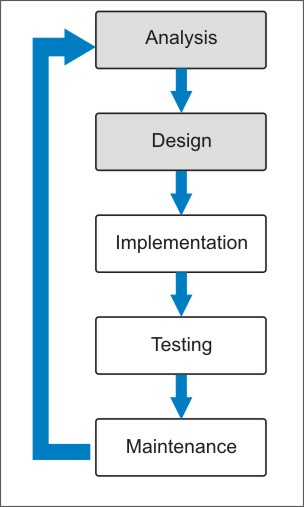
\includegraphics[width=0.6\textwidth]{images/lifecycle.jpg}
\caption{Software Development lifecycle}
\label{fig:lifecycle}
\end{figure}

\subsection{Code Generation}

When developing software, many bugs and errors occur due to coding mistakes in the implementation phase. This can happen due to reusing old software components, unimplemented methods, uninitialized variables, etc. In order to prevent those mistakes, we have to fall back onto coding standards in the development of software systems.
\\ \\
A possible approach is the use of code generation. Among the problems described earlier, it can prevent errors that emerge in manually created code. Usually, a model (e.g. in UML) serves as a blueprint for the generation of the code. Sometimes the code generated from a UML diagram is not complete and merely offers stubs to the users that still have to be implemented manually. The main reason for this is that UML is a generic modeling language. However, if we constrain the required system to a restricted domain, we are able to generate specific code from a DSL. 

\section{Contribution}

\subsection{Aims and Objectives}

The goal of this Master's Thesis is to provide a coherent modeling framework for the creation of collaborative applications running on the Android platform. 
\\ \\
These are the main objectives of the study:

\begin{itemize}
\item{Discuss the shortcomings of two-level modeling and why we need multi-level modeling}
\item{Analyze the possibilities of domain-specific modeling in the context of the Android platform}
\item{Analyze and define the different types of collaboration methods}
\item{Create a coherent framework that allows the creation of collaborative Android applications}
\end{itemize}

\subsection{Research Questions}

The research questions are sustained on underlying hypotheses. The following are the main hypotheses with accompanying research questions:

\begin{itemize}
\item{Hypothesis 1. Android is an open source software stack. \\
Research Question 1. How can we leverage the Android stack to support the modeling of Android applications?}
\item{Hypothesis 2. There exists a categorization of different types of collaboration. \\
Research Question 2. How can we support the different types of collaboration in a modeling framework?}
\item{Hypothesis 3. We have a broad offering of collaborative applications and functionalities are offered as separate applications. \\
Research Question 3. How can we integrate different functionalities in one collaborative application that is adaptable to a group of (non-technical) people?}
\end{itemize}

\subsection{Expected Outcomes}

These are the expected outcomes for this thesis:

\begin{itemize}
\item{A study of the possibilities of multi-level meta-modeling.}
\item{A study of the possibilities of modeling Android applications.}
\item{A standardization of collaborative patterns in a framework.}
\item{A description and design of a modeling framework for collaborative applications.}
\item{A case study application that shows the capabilities of the collaborative modeling framework.}
\end{itemize}

\section{Thesis Outline}

This document starts with an overview of the fundamentals of domain specific modeling in chapter 2. It also explains why there are shortcomings in the two-level modeling approach. Chapter 3 continues with a solution (multi-level modeling) that resolves problems inherent to two-level modeling. We illustrate these problems using the Metadepth multi-level modeling framework. In chapter 4, the main components of Android are discussed, such as Activities and the AndroidManifest file that is a blueprint for Android components in an application. Chapter 5 discusses the different collaborative methods such as Groupware, Computer-Supported Cooperative Work (CSCW) and Computer-Supported Collaborative Learning (CSCL). Using the concepts we have learned from chapter 5, we can make a complete framework with the appropriate collaborative patterns included in chapter 6. This chapter will contain all the designs that make the entire collaborative modeling framework. Chapter 7 proposes a case study where we have developed a complete application using the collaborative modeling framework. The application allows a group of users to authenticate (and thus initiate a session) and collaborate with each other on a certain research project. They can communicate asynchronously (by adding list items or comments on research papers) as well as synchronously (chatting). Finally, chapter 8 concludes the thesis and talks about future work.
